\section{Results}
\label{sec:Evaluation}
We collected data from $9$ subjects, each using our instrumented visualization for approximately $50$ minutes on a series of structured and unstructured tasks. We used the collected data to test the validity and effectiveness of collecting eye-tracking data in visualization space in two ways. 

First, we compared the similarity of our algorithm output to human annotation data, with the similarity between human annotations. We found that our results were on average as similar to human annotations as human annotations were similar to each other. Moreover, we conducted this analysis for all three viewed detection algorithms described in Sections~\ref{sec:AOIBasedViewedObjectDetection} to~\ref{sec:MehthodsIntelligentAlgorithm} and showed that the AOI based method (Section~\ref{sec:AOIBasedViewedObjectDetection}) performs poorly compared to the other two, and that the prediction component (Section~\ref{sec:MehthodsIntelligentAlgorithm}) improves detection accuracy by about $4\%$  (Figure~\ref{fig:quantitative}). 

Second, we demonstrate that our instrumentation method can provide relevant information by showing that viewed objects detected by our instrumentation align with the tasks we asked people to do. Moreover, we show that data collected in this way can be useful in analyzing visual behavior for data visualization users.  

We discuss the validity and benefits of these evaluation choices are discussed in Section~\ref{sec:Discussion}.

\subsection{Study Design }
\label{sec:EvalStudyDesign}

\textbf{Setup: } We used the visualization and data described in Section~\ref{sec:Methods}, and a lightweight $60$Hz EyeX eye-tracker from Tobii connected to a 17'' monitor. Subjects were seated approximately $30''$ away from the display. 

\textbf{Subjects:} We collected data from $9$ graduate and undergraduate students with ages ranging between $20$ years and $30$ years. Six of them were male and three were female. Subjects were paid $\$10$ for their participation. 

\textbf{Protocol:} Subjects were first given a description of the study's purpose and protocol. They were then introduced to our IMDB PivotPaths visualization and asked to perform a few training tasks to help them get accustomed with the visualization. This introductory part lasted on average $10$ minutes. The main section of the study followed, involved multiple instances of four types of tasks, and lasted approximately $50$ minutes. 


\textbf{Tasks:} We asked subjects to complete four types of tasks. We aimed to balance structured tasks and unstructured tasks. To solve the structured tasks, subjects had to consider a set of objects that was better defined and less variable than in unstructured tasks. This made it easier for us to test the degree to which our detection of viewed objects is aligned with the data required to complete the tasks. On the other hand, data collected for unstructured tasks may be better at informing designs of future analysis systems of such data. We limited the time we allowed subjects to spend on each task. This was done for two reasons: to limit the total duration of the study, and to make results comparable across time and users.

\begin{itemize}
\item \textbf{Task1 (structured):} Finding four commonalities between pairs of movies. The tasks were limited at three minutes each, and subjects solved the following four instances of this task: (i) Goodfellas and Raging bull; (ii) Raiders of the Lost Ark and Indiana Jones and the Last Crusade; (iii) Invictus and Million Dollar Baby; (iv) Inception and The Dark Knight Rises.  
\item \textbf{Task2 (structured):} Ranking collaborations between a director and three actors ($2$ minutes).  Subjects complete four task instances centered around the following directors: Ang Lee, Tim Burton, James Cameron and David Fincher; 
\item \textbf{Task3 (semi-structured):} Given three movies, subjects were asked to recommend a fourth ($5$ minutes). Subjects solved three such tasks: (i) Catch Me If You Can, E.T. the Extra-Terrestrial, and Captain Phillips; (ii)To Kill a Mockingbird, The Big Country, and Ben-Hur; (iii) Inglourious Basterds, The Avengers, and Django Unchained.



\item \textbf{Task4 (unstructured):} Given a brief and incomplete description of the ``Brat Pack'', a group of young actors popular in the 80's, subjects were asked to find additional members and movies they acted in. Subjects solved one such task, in approximately $5$ minutes. 
\end{itemize}


\subsection{Results}
\subsubsection{Data collected automatically is similar to that of human annotators}
\label{sec:EvalResults}


We wished to determine the degree to which the outputs of the three algorithms described in Section~\ref{sec:AOIBasedViewedObjectDetection},~\ref{sec:ProbabilisticObjectDetection}, and~\ref{sec:MehthodsIntelligentAlgorithm} (AOI, probabilistic, and intelligent) are comparable to annotation data obtained from human coders who inspected screen-captures with overlaid gaze samples and manually recorded what subjects looked at. Using a methodology described in the following paragraph, we found that overlaps between the annotations of human coders and the outputs of the intelligent algorithm for the same input, are close to overlaps between the coders' own annotations. We also found that the intelligent algorithm outperforms the probabilistic and AOI ones. The detailed results are shown in Figure~\ref{fig:quantitative}.

Specifically, we enlisted the help of five coders and asked them to annotate eye-tracking data corresponding to one task of approximately three minutes, for each of six subjects.  The task was the same for all coders – task 1.ii. The six subjects were selected randomly and were the same for all five coders. Coders spent approximately one hour per subject completing this task. Four coders completed all six assigned tasks, while one was able to annotate only three of the six data sets. 

Coders used an application that allowed them to browse through screen captures of a users' activity with overlaid gaze coordinates. We asked coders to advance through the videos in $100$ms time-steps, determine what visual objects their assigned subjects were viewing, and record those objects along with the start and end time of their viewing. If unsure which of multiple objects was viewed, coders were were allowed to record all of them.  

We transformed this data into temporal vectors at $100$ms resolution. Thus, these vectors contained at each position one or several objects that were likely viewed by a subject during the $100$ms time-step which corresponded to that position. We then created similar representations from our automatically collected data. We defined a similarity measure between two such vectors as the percentage of temporally aligned cells from both that were equal. Equality between cells was defined as a non-empty intersection between their contents. 

To determine the overlap between algorithm output and human annotations, we computed the similarity of the algorithm's output for each subject's data to each of the coders' annotation of the same data.  This yielded $1$ algorithm $\times$ $4$ coders $\times$ $6$ subjects $+$  $1$ algorithm $\times$ $1$ coder $\times$ $3$ subject $=$ $27$ similarities per algorithm. We averaged these similarities and plotted them as the first three bars in Figure~\ref{fig:quantitative}. To determine the overlap between the coders' own results, we computed the similarity between each coder's own annotation of a subject's data to all other available annotations of the same data. Since for three subjects we had five annotations ($3$ subjects $\times$ $10$ annotation pairs $=$ $30$ similarities) while for the remaining three we only had four ($3$ subjects $\times$ $6$ annotation pairs $=$ $18$ similarities) this yielded $48$ similarities, which we averaged and plotted as the last bar of Figure~\ref{fig:quantitative}.

The data we collected allowed us to perform this analysis for all three algorithms described in Section~\ref{sec:MethodsAlgorithmsViewedObjectDetection}. Specifically, if we only consider gaze scores $gs$ (Section~\ref{sec:AOIBasedViewedObjectDetection}) equal to one, we essentially have the output of the AOI based approach. If we limit the analysis to $gs$ scores alone, without the prediction component described in Section~\ref{sec:MehthodsIntelligentAlgorithm}, we have the output of the probabilistic approach described in Section~\ref{sec:ProbabilisticObjectDetection}.

\begin{figure}[htb]
  \centering
  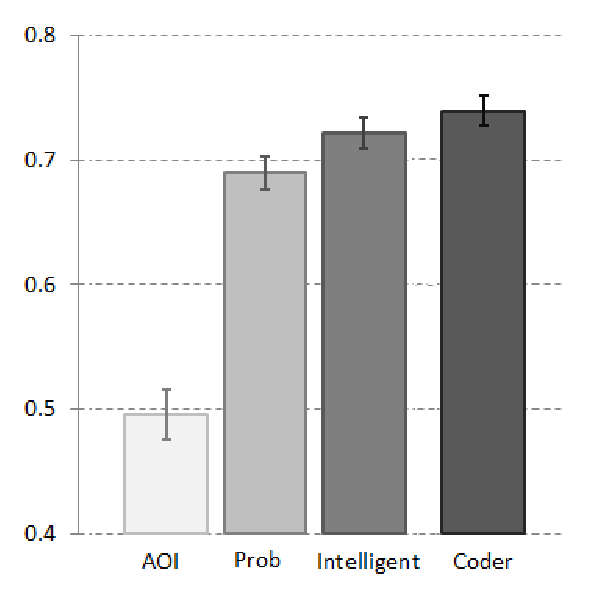
\includegraphics[width=0.6\linewidth]{images/algosComparison.eps}
  \caption{Comparison between automated and manual viewed object detection. The first three bars show the overlap between the outputs of the three algorithms described in Section~\ref{sec:AOIBasedViewedObjectDetection},~\ref{sec:ProbabilisticObjectDetection}, and~\ref{sec:MehthodsIntelligentAlgorithm} and annotation results of human coders. The last bar shows the overlap within the human annotators' own results. Values correspond to averages over multiple tasks, multiple subject data sets, and multiple annotators, and are computed as described in Section~\ref{sec:EvalResults}. Error bars extend by one standard error.}
	\label{fig:quantitative}
\end{figure}


\subsubsection{Data collected automatically is relevant and useful}
\label{sec:EvalDataCollected}
We used two visual representations and analyses to show that data collected automatically using our approach are tightly correlated with the tasks that users had to do. We chose this evaluation for two reasons. First, it provides evidence that the automatic instrumentation approach can be used to solve the inverse problem: an observer or analyst who is unfamiliar to a subject's intentions can determine what these are by looking at the subject's visual interest in particular data. 

Second, it demonstrates how the automated collection of eye-tracking data can facilitate novel analyses and insights into how users perform tasks in a visualization. For example, our approach allowed us to quantify that a user's interest in a visual item, even if present on the screen, decays exponentially with a decrease in that item's relevance to the user's task. While it was generally known that users follow ``information scent'' when solving tasks visually [x], it was never quantified exactly how focused users' perception really is.

\textbf{First}, we created heatmap representations from our collected data (Figure~\ref{fig:heatmap}) to illustrate qualitatively the strong connection between the tasks our subjects were asked to perform and the data we collected from them. We listed viewed objects vertically and discretized viewing scores, using averaging, into $500ms$ intervals, which we arranged horizontally. Thus, time is shown horizontally, viewed objects vertically, and intensity of heatmap cells indicate the degree to which an object was viewed at a given moment in time. The viewed objects listed vertically were colored based on their type (movie, actor, director, genre) and could be sorted by either first time they were viewed, amount of viewing activity, or type.

Figure~\ref{fig:heatmap}, left, shows the results for a subject performing the second instance of task 1 (task 1.ii): finding commonalities between two Indiana Jones movies (see Section~\ref{sec:EvalStudyDesign}). In the top panel, the heatmap is ordered by the amount of visual attention that the subject dedicated to each element in the visualization. We notice that elements at the top of the heatmap are tightly connected to the subject's  task.   In the bottom panel, viewed items are ordered by category (genre, director, movie, actor). We can notice a clear temporal pattern: the movies involved directly in the task are viewed throughout the analysis, actors are considered first, then genres, then directors, and ultimately a quick scan of other movies. This pattern was observed for most of our subjects and interestingly corresponds to the ordering used in the task's phrasing: we asked subjects to determine actors, genres, and directors that were common between two movies.  

Figure~\ref{fig:heatmap}, right, shows a subject's results for one of the instances of task 3, which was significantly less structured than task 1 (see Section~\ref{sec:EvalStudyDesign}). This heatmap  was sorted by the first time each object was viewed and shows how subjects were moving through different aspects of the analysis, and revisited objects often at different moments in time. Heatmaps associated to these task types typically showed a wider range of viewed objects. We attribute this pattern to the more exploratory nature of the tasks.  

\begin{figure*}[!ht]
  \centering
  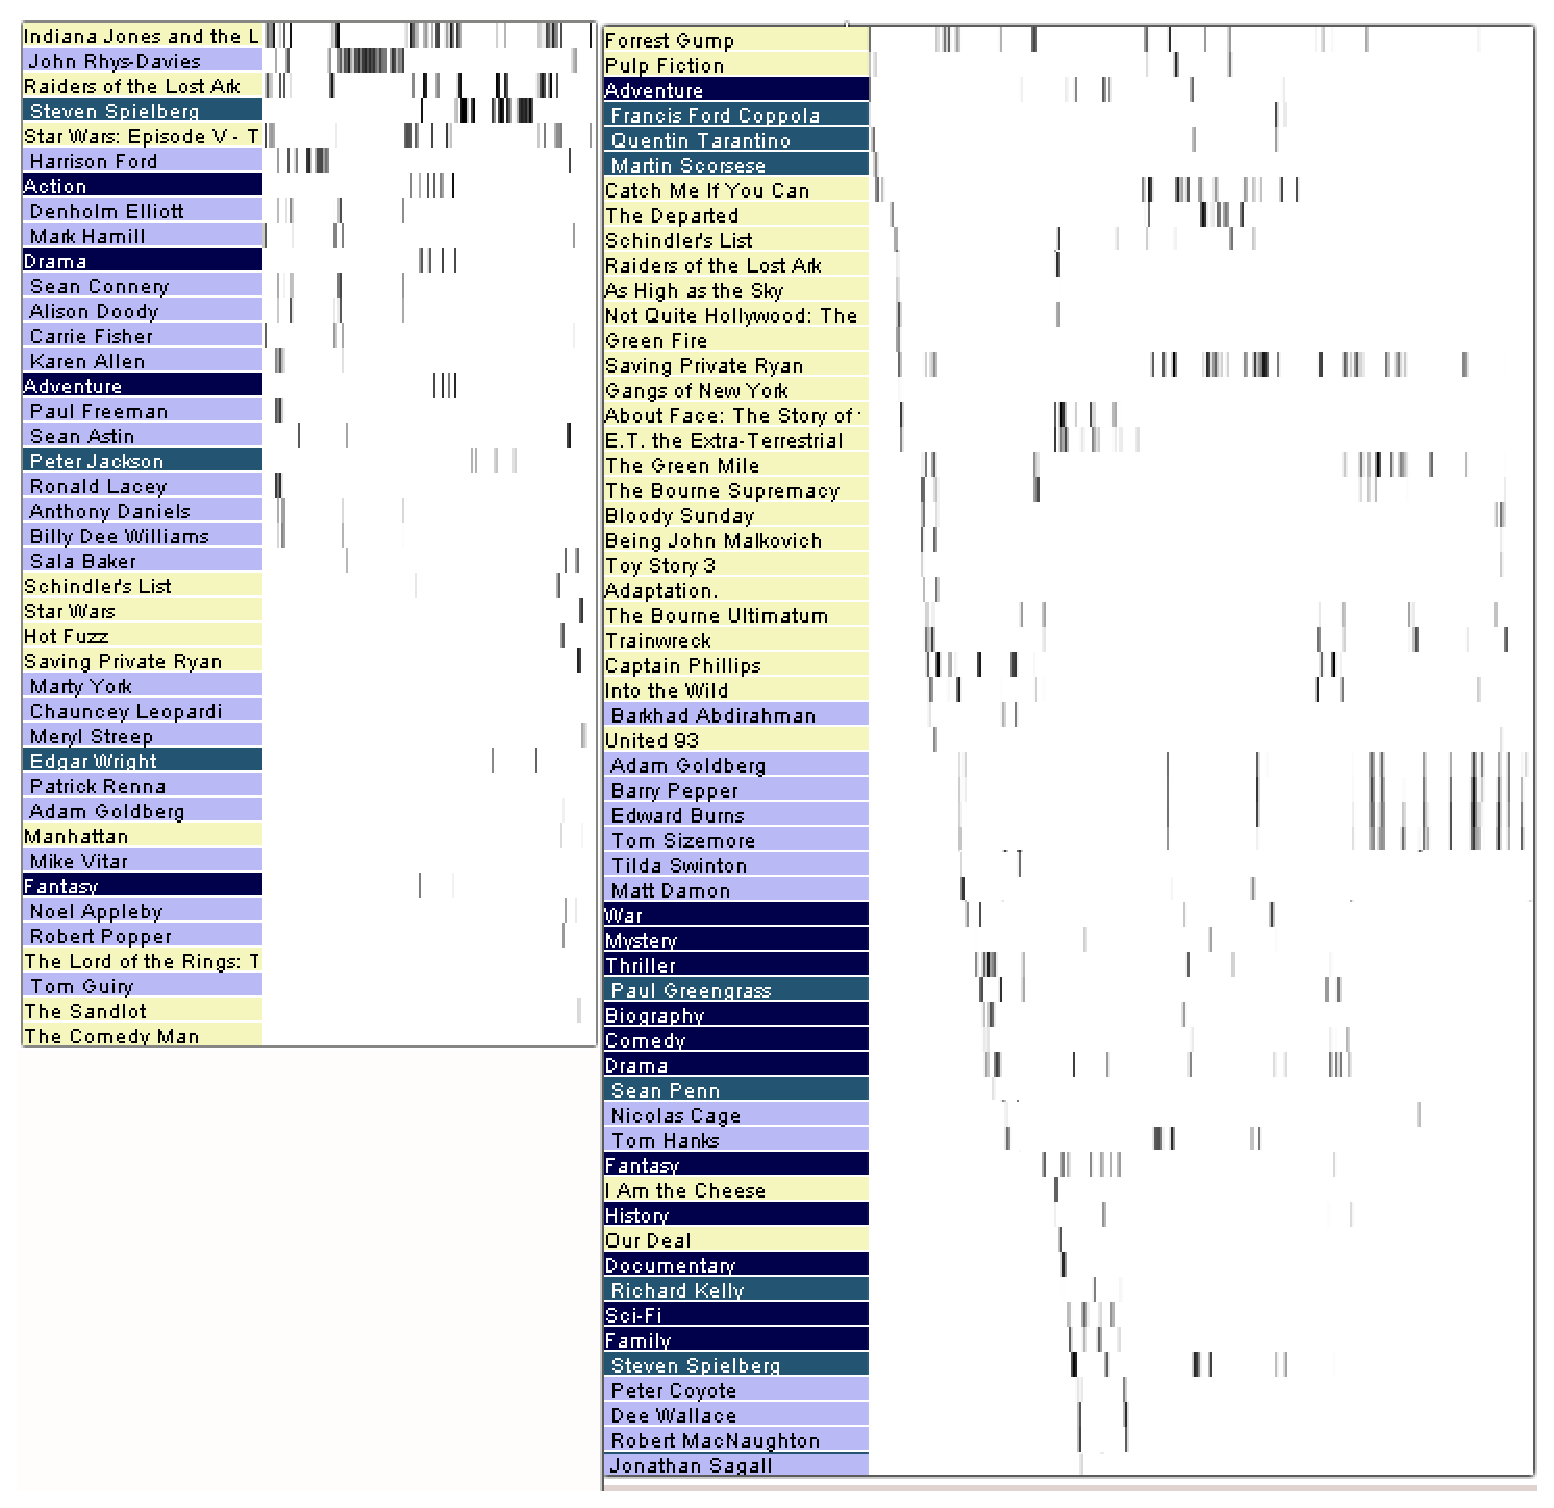
\includegraphics[width=0.75\linewidth]{images/heatmaps.eps}
  \caption{Heatmap views of one subject's activity on two tasks; time, in 500ms increments, are shown horizontally; viewed objects are viewed vertically; cell darkness indicates viewing intensity (black: high; white: low). (Top left) Data for the task 1.ii (see Section~\ref{sec:EvalStudyDesign}); viewed items are ordered by decreasing total amount they were viewed. (Bottom left) Data for the task 1.ii (see Section~\ref{sec:EvalStudyDesign}); viewed items are ordered by category (genre, director, movie, actor). (Right) Data for the task 1.ii (see Section~\ref{sec:EvalStudyDesign} 4.1); viewed items are ordered by first time they were seen. 
}
	\label{fig:heatmap}
\end{figure*}


\textbf{Second}, in a more quantitative approach, we formalized the relevance of each visual item to a particular task and plot this relevance against the amount of interest that each item attracted, as shown in Figure~\ref{fig:RelevanceDiagram}. These plots illustrate the degree to which task relevance impacts the amount that each visual item is tended to by subjects, and demonstrates that our instrumentation captures relevant data.  

We formalize the relevance of a visual item to a task as $\text{relevance} = \frac{1}{(1+d)}$ where $d$ is the shortest graph-distance between that item and any item mentioned in the task description.  To exemplify, the relevance of Goodfellas and Ranging Bull to tasks 1.i is $1$ because they are the focus of the task, that of Martin Scorsese is $\frac{1}{2}$ because he directed both movies, while that of other movies directed by Scorsese are assigned a relevance of $\frac{1}{3}$ because they are only indirectly connected to Goodfellas and Raging Bull, through Martin Scorsese. This definition is not complete as items might be relevant to a task even though they are not directly mentioned in the description.  For instance, items that eventually constitute a subject's answer will elicit more of the subject's attention. Moreover, this definition is particular to the visualization we instrumented.

A few insights can be drawn from analyzing Figure~\ref{fig:RelevanceDiagram}. First, even though many items were shown to subjects during their tasks, only very few were viewed for significant periods of time, and many were not viewed at all. In fact, the interest in a particular item drops exponentially with that item's relevance to the task, which aligns with knowledge that people's perception is goal-driven.  Second, the types of data that users view more are correlated to the particularities of each task. For example, task 3 involved movie recommendations and Figure~\ref{fig:RelevanceDiagram}(c) illustrates that genres and directors were viewed significantly more than in task 4, which involved determining the identity of a group of actors, and, as shown in  Figure~\ref{fig:RelevanceDiagram}(d), drove users to mostly focus their attention on actors. 



\begin{figure}[!htb]
  \centering
  \includegraphics[width=0.9\linewidth]{images/RelevanceDiagramTask1.eps}
	
	\includegraphics[width=0.61\linewidth]{images/RelevanceDiagramTask2.eps}
	
	\includegraphics[width=0.71\linewidth]{images/RelevanceDiagramTask3.eps}
	
	\includegraphics[width=\linewidth]{images/RelevanceDiagramTask4.eps}
	
  \captionof{figure}{Users' interest in data objects, in relation to each objects' relevance to a task, for twelve tasks of four types. Each individual task is plotted in its type's corresponding chart as a subdivision across multiple relevance categories. Relevance was computed as described in Section~\ref{sec:EvalDataCollected}, and plotted for all objects that were visible to subjects during each task. The average interest in objects with the same task relevance are linked by separate polylines for each individual task; errors bars extend from the averages by one standard error.}
	\label{fig:RelevanceDiagram}
\end{figure}





\subsubsection{Assumptions about viewing transition patterns hold}
We analyzed common viewing-transition patterns in the data we collected. Examples include how often our subjects change views from a genre to an un-highlighted item versus to a highlighted one, or how often subjects transition between connected items and unconnected items. The data is summarized in the last columns  (real transitions) of the panels in Table~\ref{tab:TransitionFromMovie}, and shows that the assumptions we made informally in Section~\ref{sec:Methods}, that users show a preference to transition their view to connected or highlighted items, holds. For example, the first panel in Table~\ref{tab:TransitionFromMovie} shows that after looking at a movie, users were five times more likely to look at an actor connected to that movie ($prob. = 0.019$), and more than twently times more likely to look at an actor that was both connected to the movie and highlighted ($prob. = 0.089$), than a random other actor ($prob. = 0.004$).  


To compute these numbers, we first discarded the prediction component from our collected data, since the prediction represents exactly the assumption we try to test, and would have thus biased the data. We then counted direct viewing transitions between all types of objects to all other types of objects, and we separated transitions to connected objects and to highlighted objects from all other ones, as seen in the first columns in Table~\ref{tab:TransitionFromMovie}.  For example, after looking at a movie title, our users looked at an actor that was unconnected to that movie and unhighligted $793$ times; at the same time they looked at an actor that was connect to the movie and highlighted $616$ times. To understand the row headers in Table~\ref{tab:TransitionFromMovie} it is important to note that in our viusalization only movies were connected to actors, genres, and directors, while in these in turn were not connected to each other. Thus, the two options of transitioning to (1) a connected and (2) a highlighted and connected item exist only when tranisitoning to and from movies.    

These transition counts were first translated into raw transition probabilities by normalizing transition numbers in each category by the total number of transitions in each panel. For example , from a total of $10459$ transitions from a movie to any other item (listed at the bottom at the first panel in Table~\ref{tab:TransitionFromMovie}, $5727$ were to unhighlighted movies, yielding a transition probability of $5727 / 10459 = 0.548$.

However, these raw transition probabilities are misleading because they assume that after viewing a particular item, a user can chose the next item to view with equal opportunity from each of the considered categories (e.g., actor, movie, unconnected, connected, highlighted). This however, is not true: when a subject transitions their gaze from a source to a target, the visualization typically contains many more items that are not highlighted and are unconnected to the source, than those that are. For example, even though we observed 793 transitions from a movie to an unconnected actor, and just 228 to a connected one, the visualization provided many more opportunities for a user to view an unconnected actor after a movie than a connected one.

Assume the following simplified case: a movie is connected to two of ten actors shown in the visualization. We observe that of ten transitions from that movie to one of the ten actors, five were to one of the two connected actors, while the other five were to the remaining eight unconnected actors. The raw probabilities would in this case be equal, at $5/10 = 0.5$, and may not immediately suggest a preferance for transitions to connected items over unconnected items. However, if there was no transitioning preference to either connected or unconnected items, the probability of transitioning to any actor would be equal at $0.1$, that of  transitioning to a connected one would be $0.2$, as there are two connected actors, while that of transitioning to an unconnected actor would be $0.8$. Thus, observing an equal number of transitions to connected and unconnected items indicates in fact a strong preferance for connected items. More specifically, the observed transition probability from a movie to a connected actor is $0.5/0.2=2.5$ times higher than the unbiased probability, while the oberserved transition probability from a movie to an unconnected actor is a fraction of ($0.5/0.8=0.625$) of the unbiased one.  These unbiased probabilities and ratios between observed probabilities and unbiased probabilities are displayed in the last two columns of Table~\ref{tab:TransitionFromMovie}. 

To compute this elements, every time we counted a transition from a source to a target, we also counted all options available to a user at that point, given the state and structure of the visualization at the time of transition. In our simplified example, this means that for each of our ten observed transitions we would count two possible transitions to connected actors and eight possible transitions to unconnected actors, ending up with $20$ counts for connected actors, and $80$ counts for unconnected actors. These counts allow us to at the end to compute the two unbiased probabilities as $20/(20+80)$ and $80/(20+80)$. In our real visualization, for each observed transition from a source, we had to recreate the state of the visualization at the time of the transition, and count the number of objects in each category (e.g., actors highlighted and connected to the source, actors un-highlighted but connected to the source, actors un-highlighted and unconnected to the source, etc.)  

A quick inspection of the contents of Table~\ref{tab:TransitionFromMovie} will show that the assumptions we made in Section~\ref{sec:Methods} hold. Moreover, this type of analysis can be useful in helping us understand how visualizations are used and how workflows are approached by users.

\begin{table}[htbp]	
	\centering
		\begin{tabular}{|c|c|c|c|c|c|}
			\hline
			 \multicolumn{2}{ |c| }{Movie to}  &\shortstack{No. of\\transitions} 	&\shortstack{ Observed \\transition\\probability }	&\shortstack{	 Unbiased\\transition\\probability} & \shortstack{Ratio \\$\frac{\text{Observed}}{\text{Unbiased}}$}\\ \hline
      \multirow{4}{*}{Actor}	&-	&793	&0.076	&0.004& 19	\\	\cline{2-6}
															&H	&147	&0.014	&0.032	&0.44	\\	\cline{2-6}
															&C	&228	&0.022	&0.019	&1.16	\\	\cline{2-6}
															&CH	&616	&0.059	&0.089	&0.66	\\	\hline
				\multirow{2}{*}{Movie}	&-	&5727	&0.548	&0.131	&4.18	\\	\cline{2-6}
																&H	&1798	&0.172	&0.368	&0.47	\\	\hline
				\multirow{4}{*}{Director}	&-	&304	&0.029	&0.01	&2.9	\\	\cline{2-6}
																	&H	&37	&0.004	&0.051	&0.08	\\	\cline{2-6}
																	&C	&51	&0.005	&0.027	&0.19	\\	\cline{2-6}
																	&CH	&174	&0.017	&0.135	&0.13	\\	\hline
				\multirow{4}{*}{Genre}	&-	&193	&0.018	&0.005	&3.6	\\	\cline{2-6}
															&H	&40	&0.004	&0.027	&0.15	\\	\cline{2-6}
															&C	&69	&0.007	&0.015	&0.47	\\	\cline{2-6}
															&CH	&282	&0.027	&0.087	&0.31	\\	\hline
					\multicolumn{2}{ |c| }{Total}	&10459	&1	&1	&1	\\
				\hline
		\end{tabular}		
		%\caption*{(a)Transitions from Movies}
		\smallskip
		
		\begin{tabular}{|c|c|c|c|c|c|}
			\hline
			 \multicolumn{2}{ |c| }{Actor to}    &\shortstack{No. of\\transitions} 	&\shortstack{ Observed \\transition\\probability }	&\shortstack{	 Unbiased\\transition\\probability} & \shortstack{Ratio \\$\frac{\text{Observed}}{\text{Unbiased}}$}\\ \hline
						 \multirow{2}{*}{Actor}	&-	&4711	&0.533	&0.032	&16.66	\\	\cline{2-6}
																		&H	&2164	&0.245	&0.372	&0.66	\\	\hline
							\multirow{4}{*}{Movie}	&-	&839	&0.095	&0.031	&3.06	\\	\cline{2-6}
																			&H	&213	&0.024	&0.113	&0.21	\\	\cline{2-6}
																			&C	&386	&0.044	&0.157	&0.28	\\	\cline{2-6}
																			&CH	&352	&0.04	&0.236	&0.17	\\	\hline
							\multirow{2}{*}{Director}	&-	&68	&0.008	&0.003	&2.67	\\	\cline{2-6}
																				&H	&29	&0.003	&0.034	&0.09	\\	\hline
							\multirow{2}{*}{Genre}	&-	&43	&0.005	&0.002	&2.5	\\	\cline{2-6}
																			&H	&39	&0.004	&0.02	&0.2	\\	\hline
								\multicolumn{2}{ |c| }{Total}&8844	&1	&1	&1	\\
	\hline

		\end{tabular}
	%\caption*{(b)Transitions from Actors}
	\smallskip
	
	\begin{tabular}{|c|c|c|c|c|c|}
			\hline
			 \multicolumn{2}{ |c| }{Director to}   &\shortstack{No. of\\transitions} 	&\shortstack{ Observed \\transition\\probability }	&\shortstack{	 Unbiased\\transition\\probability} & \shortstack{Ratio \\$\frac{\text{Observed}}{\text{Unbiased}}$}\\ \hline
       \multirow{2}{*}{Actor}	&-	&71	&0.042	&0.001	&42	\\	\cline{2-6}
															&H	&24	&0.014	&0.011	&1.27	\\	\hline
			\multirow{4}{*}{Movie}	&-	&271	&0.162	&0.031	&5.23	\\	\cline{2-6}
															&H	&55	&0.033	&0.121	&0.27	\\	\cline{2-6}
															&C	&130	&0.077	&0.108	&0.71	\\	\cline{2-6}
															&CH	&93	&0.055	&0.139	&0.4	\\	\hline
			\multirow{2}{*}{Director}	&-	&384	&0.229	&0.054	&4.24	\\	\cline{2-6}
																&H	&160	&0.095	&0.299	&0.32	\\	\hline
			\multirow{2}{*}{Genre}	&-	&256	&0.153	&0.026	&5.88	\\	\cline{2-6}
															&H	&234	&0.139	&0.211	&0.66	\\	\hline
				\multicolumn{2}{ |c| }{Total}	&1678	&1	&1	&1	\\
				\hline
		\end{tabular}
		%\caption*{(c)Transitions from Director}
		\smallskip
		
		\begin{tabular}{|c|c|c|c|c|c|}
			\hline
			 \multicolumn{2}{ |c| }{Genre to}   &\shortstack{No. of\\transitions} 	&\shortstack{ Observed \\transition\\probability }	&\shortstack{	 Unbiased\\transition\\probability} & \shortstack{Ratio \\$\frac{\text{Observed}}{\text{Unbiased}}$}\\ \hline
       \multirow{2}{*}{Actor}	&-	&61	&0.03	&0.0005	&60	\\	\cline{2-6}
															&H	&32	&0.016	&0.011	&1.45	\\	\hline
				\multirow{4}{*}{Movie}	&-	&229	&0.113	&0.012	&9.42	\\	\cline{2-6}
																&H	&46	&0.023	&0.077	&0.3	\\	\cline{2-6}
																&C	&172	&0.085	&0.024	&3.54	\\	\cline{2-6}
																&CH	&138	&0.068	&0.135	&0.5	\\	\hline
				\multirow{2}{*}{Director}	&-	&282	&0.139	&0.015	&9.27	\\	\cline{2-6}
																	&H	&195	&0.096	&0.383	&0.25	\\	\hline
				\multirow{2}{*}{Genre}	&-	&348	&0.172	&0.013	&13.23	\\	\cline{2-6}
																&H	&526	&0.259	&0.328	&0.79	\\	\hline
					\multicolumn{2}{ |c| }{Total}	&2029	&1	&1	&1	\\
			\hline
		\end{tabular}
		%\caption*{(d)Transitions from Genres}\smallskip
	\captionof{table}{Transitions from a source object to a target object, divided by: (i) type of source and target; (ii) whether the target was highlighted (H); (iii) whether the target was highlighted and connected to the source (HC); (iv) and whether source and target were neither highlighted nor connected. Columns show: (i) the number of direct transitions for the source/target combination; (ii) the observed transition probability from the source to that target; (iii) the (unbiased) probability of transition between source and target if all elements had equal probability to be viewed; (iv) the ratio between observed and unbiased transition probabilities.}
	\label{tab:TransitionFromMovie}
\end{table}